\section{•}
\label{•}

Bei dem Wärmeentzug aus einem Raum durch einen Vedampfer kommt es zu mehreren thermodynamischen Phänomenen. Die auftretenden Phänomene lassen sich in folgende Gruppen einordnen:

\begin{itemize}
\item	Abkühlung der feuchter Luft 
\item	Bereifung- und Eisbildung des Verdampfers.
\end{itemize}

In den nachfolgenden Abschnitten \ref{subsec:Reif- und Eisbildung} und \ref{subsec:Morphologie} werden die Phänomene kurz erklärt und in Kontext zu dieser Arbeit gestellt. 

\subsection{Feuchte Luft}
\label{subsec:Feuchte Luft}

Der Verdampfer hat die Aufgabe einer Umgebung Energie in Form von Wärme zu entziehen, hierfür wird in einem Wärmeübetrager flüssiges Kältemittel verdampft. Das verdampfende Kältemittel entzieht zunächst dem Wärmeübertrager die Wärme. Danach entzieht der Wärmeübertrager über seine Lamellen der vorbeiströmenden Luft Wärme. 
Bevor sich Reif oder Eis auf einem Verdampfer bildet, wird zunächst die noch nicht gesättigte feuchte Luft abgekühlt. Luft besitzt die Eigenschaft Wasser aufnehmen zu können. Warme Luft kann mehr Wasser aufnehmen als kalte Luft. Diese Beladung ist definiert als 

\begin{equation}

\label{Beladung}
\end{equation}



\subsection{Reif- und Eisbildung}
\label{subsec:Reif- und Eisbildung}

\begin{figure}[htb]
\centering		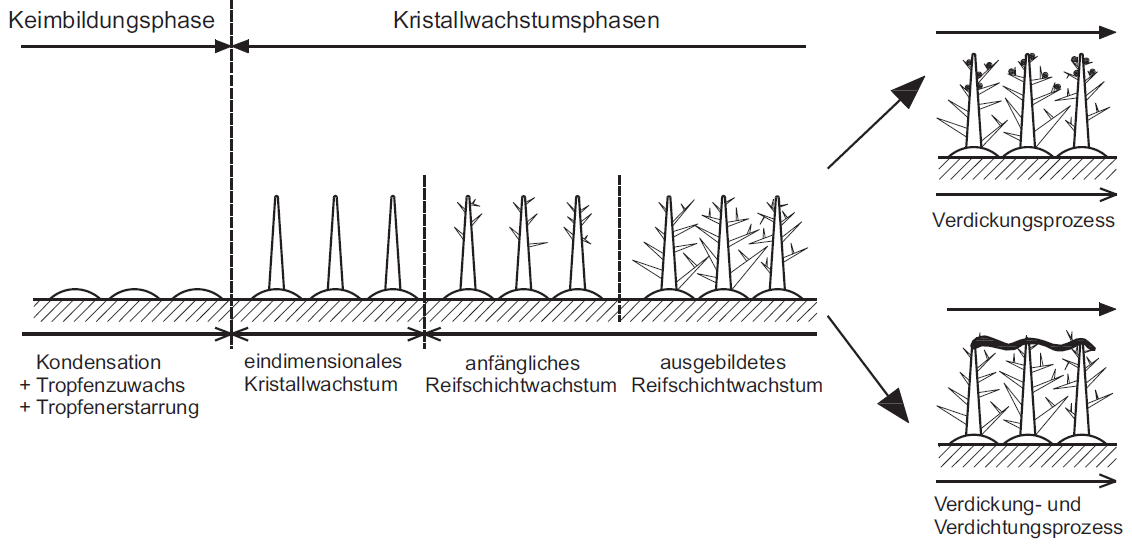
\includegraphics[width=0.85\textwidth]{Pictures/Reifbildungsphasen_Schydlo.png}
\caption{Kristallwachstum auf einer ebenen Oberfläche \citep{Schydlo2010}}
\label{fig:einfacher Kältekreislauf}
\end{figure}

